{\textbf{{1. IP数据报首部格式分析}}}

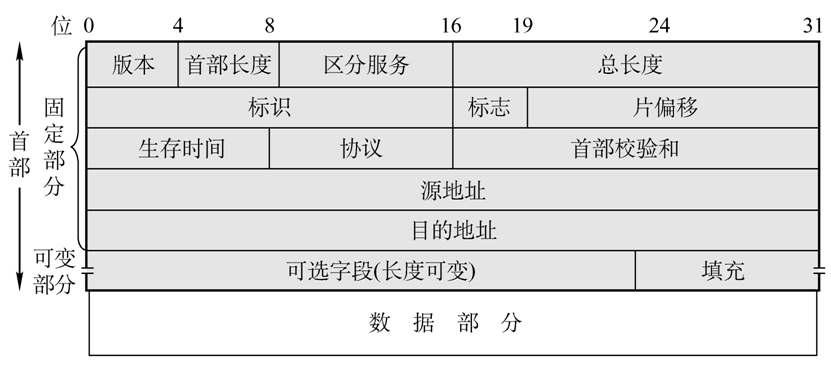
\includegraphics[width=3.33333in,height=1.47917in]{png-jpeg-pics/A9081B07899EF05DB05E89AD0FA5206C.png}

\textbf{1.
版本。}占4位,就是说这个IP数据报是IPv4版本还是IPv6版本,通信双方的版本必须一致。

\textbf{2.
首部长度。}占4位,IP数据报的首部实际上是60B(但是有40B基本从不使用,考试的时候就认为IP数据报的首部是20B,绝对不会错),前面也讲过IP数据报首部的长度必须是4B的倍数,这样就只要用15个标记(每个标记4位)就可以表示60B。

\textbf{3. 区分服务。}占1B,从没使用过,不会考,可忽略。

\textbf{4.
总长度。}占2B,{\textbf{千万不要和首部的基本长度弄混淆,这里的基本单位长度是1B,不再是4B,并且总长度包括了首部和数据部分}},很明显16位可以表示的长度为65535B(因为16位表示的数的范围是0~65535)。

\textbf{5. 标识。}占2B,它是一个计数器,用来产生IP数据报的标识。

\textbf{6. 标志。}占3位,目前只有前2位有意义,即MF和DF。

\textbf{7.
片偏移。}占13位,前面已经讲过,但是需要注意的是片偏移是8B的整数倍。

\textbf{8.
生存时间。}占8位,如果一个数据报一直在网络中转圈,网络资源就被白白浪费了,所以需要设置生存时间(Time
To Live,TTL),即数据报在网络中可通过的路由器数的最大值。

\textbf{9.
协议。}占8位,当接收端收到数据报时,肯定要交付给传输层的某种协议去处理,是交给传输层的TCP协议,还是交给传输层的UDP协议,需要此标志给出。

\textbf{10.
首部校验和。}占16位,只需记住只检验数据报的首部,不检验数据部分。

\textbf{11. 源地址。}发送端主机的IP地址,即源地址。

\textbf{12. 目的地址。}接收端主机的IP地址,即目的地址。
